\documentclass[../../../main.tex]{subfiles}
    
    \lstset{basicstyle=\small,
      showstringspaces=false,
      commentstyle=\color{black},
      keywordstyle=\color{blue}
    }
    
    \graphicspath{{images/Stromversorgung/}{../../../images/Stromversorgung/}{../../images/Stromversorgung/}}

    \begin{document}
    \subsection{Stromversorgung}
    In der Aufgabenstellung ist gefordert, dass die Antriebsenergie über die Schienen bezogen wird. Von diesem Strom muss mindestens der Motor versorgt werden. Zusätzlich benötigt die Systemsteuerung, Sensoren und Aktoren Strom. Diese können auch über die Schienen versorgt werden oder auch über eine Zusätzliche Energiequelle (wie z.B. einen Akku) versorgt werden.
    In diesem Kaptitel werden verschiedene Konzepte beschrieben und analysiert.

    \textbf{Übersicht Konzepte}\\
    Es werden der verschiedene Möglichkeit betrachtet. Zu jeder Möglichkeit werden Vor- und Nachteile aufgelistet und Risiken analysiert. Es sind auch Kombinationen aus mehreren Varianten denkbar.

    \begin{itemize}
        \item Komplette Stromversorgung über die Schienen
        \item nur die Antriebsenergie über die Schienen, die Energie für die Systemsteuerung über einen Akku 
        \item die Antriebsenergie über die Schienen, die Energie für die Systemsteuerung über einen Akku welcher über die Schienen nachgeladen wird.
    \end{itemize}
    
    \subsubsection{Alles über die Schienen}
    Um die gesamte Energie über die Schienen zu beziehen wird mindestens ein Schleifkontakt auf jeder Schiene benötigt und die Spannung muss von den gegebenen 20V einmal für die Systemsteuerung und einmal für den Motor angepasst werden. Die Spannung für gewisse Komponenten direkt abzugreifen ist wegen der Grossen Toleranz (+/- 2V ) der Versorgung nicht möglich. Eine Stabilisierung auf eine tiefere ist in jedem Fall notwendig. 
    
    \begin{flushleft}
        \begin{table}[H]
        \begin{tabular}{ | l | p{11cm} |}
        \hline
        \textbf{Problemstellung} & Stromversorgung \\ \hline
        \textbf{Disziplin} & Elektrotechnik \\ \hline
        \textbf{Lösungskonzept} & Alles über die Schienen\\ \hline
        \textbf{Komponente} & \begin{itemize}
            \item Spannungsregler für Steuerung (5V)
            \item Spannungsregler für Motor (z.B. 12V)
            \item Schleifkontakte
            \end{itemize}\\ \hline
        \textbf{Bewertung} &  \begin{itemize}
                                \item[+] kleiner Platzbedarf, keine weiteren grossen Komponenten erforderlich
                                \item[+] geringe Kosten
                                \item[-] Strombegrenzung der Schienen muss für das gesamte System reichen.
                                \item[-] Gefahr von Unterbrechungen / Wackelkontakt
                                \item[-] System kann beim Aufbau erst beim Aufsetzen auf die Schienen gestartet werden. 
                              \end{itemize} \\ \hline
        \end{tabular}
        \caption{Konzeptbeurteilung: Stromversorgung Alles über die Schienen}
        \label{tab:strom_konzept_schienen}
    \end{table}
    \end{flushleft}

    \textbf{Risiken}\\
    Zu diesem Lösungskonzept werden folgende Risiken betrachtet und eingeschätzt.
    \begin{enumerate}[I]
        \item Unterbrechung der Stromversorgung durch Wackelkontakt
        \item zu Teuer
        \item zu Wenig Strom zur verfügung
        \item zu schwierig umzusetzen (unter Berücksichtigung einer späteren Änderung zu einer Alternativlösung)
    \end{enumerate}

    In Abbildung \ref{fig:strom_risikomatrix_schienen} werden die Risiken nach möglicher Schadenshöhe und Eintrittswahrscheinlichkeit eingeschätzt.

    \begin{figure}[H]
        \centering
        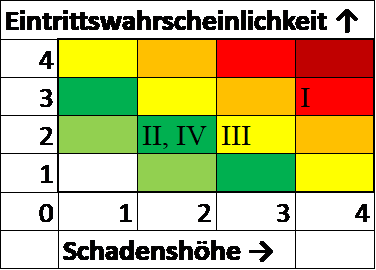
\includegraphics[width=0.4\textwidth]{Strom_Risiko_Schienen.png}
        \caption {Risikomatrix gesamte Schromversorgung über die Schienen}
        \label{fig:strom_risikomatrix_schienen}
    \end{figure}

    Hier ist besonders das Risiko für den Wackelkontakt besonders gross, da ein Unterbruch zu einem kompletten Systemabsturz führen kann. Dieses Risiko kann über eine Stützung z.B. mit einem Kondensator minimiert werden.\\
    Das Risiko der Strombegrenzung ist jedoch in der Aufgabenstellung festgelegt und lässt sich in diesem Konzept nicht minimieren.

    \subsubsection{Zusätzlicher Akku}
    In diesem Konzept werden auch mindestens zwei Schleifkontakt für die Antriebsenergie benötigt. Die Systemsteuerung wird über einen Akku gespeist. Die Spannung ab den Schienen muss wegen der grossen Toleranz der Versorgungsspannung stabilisiert werden. Die Spannung für die Systemsteuerung muss je nach Akkutyp ebenfalls stabilisiert werden.
    Der Akku muss dabei für mindestens zwei Runden auf der Teststrecke reichen.

    \begin{flushleft}
        \begin{table}[H]
        \begin{tabular}{ | l | p{11cm} |}
        \hline
        \textbf{Problemstellung} & Stromversorgung \\ \hline
        \textbf{Disziplin} & Elektrotechnik \\ \hline
        \textbf{Lösungskonzept} & Schienen für den Antrieb und zusätzlichen Akku für die Systemsteuerung\\ \hline
        \textbf{Komponente} & \begin{itemize}
            \item Spannungsregler für Steuerung (5V)
            \item Spannungsregler für Motor (z.B. 12V)
            \item Schleifkontakte
            \item Akku
            \end{itemize}\\ \hline
        \textbf{Bewertung} &  \begin{itemize}
                                \item[+] zuverlässige Stromversorgung für die Systemsteuerung
                                \item[+] System kann schon vor dem Aufbau hochgefahren werden 
                                \item[+] gesamter Strom der Schienen kann für den Antrieb genutzt werden
                                \item[-] zusätzliche Kosten für einen Akku
                                \item[-] zusätzliches Gewicht
                                \item[-] grosser Platzbedarf für den Akku 
                              \end{itemize} \\ \hline
        \end{tabular}
        \caption{Konzeptbeurteilung: Stromversorgung Schienen und Akku}
        \label{tab:strom_konzept_schienen_und_akku}
    \end{table}
    \end{flushleft}

    \textbf{Risiken}\\
    Zu diesem Lösungskonzept werden folgende Risiken betrachtet und eingeschätzt.
    \begin{enumerate}[I]
        \item Unterbrechung der Stromversorgung durch Wackelkontakt
        \item zu Teuer
        \item zu Wenig Strom zur verfügung
        \item zu schwierig umzusetzen (unter Berücksichtigung einer späteren Änderung zu einer Alternativlösung)
    \end{enumerate}

    In Abbildung \ref{fig:strom_risikomatrix_akku} werden die Risiken nach möglicher Schadenshöhe und Eintrittswahrscheinlichkeit eingeschätzt.

    \begin{figure}[H]
        \centering
        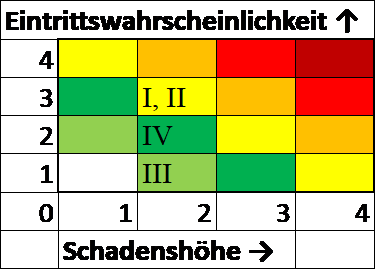
\includegraphics[width=0.4\textwidth]{Strom_Risiko_Akku.png}
        \caption {Risikomatrix Antriebsenergie über die Schienen und Akku für die Systemsteuerung}
        \label{fig:strom_risikomatrix_akku}
    \end{figure}

    Die Risiko bei einer Unterbrechung der Stromversorgung für den Motor ist geringer als bei einer Unterbrechung bei der Systemsteuerung. Das Restrisiko für den Antrieb kann jedoch noch weiter reduziert werden, wenn eine Stützung realisiert wird.


    \subsubsection{Zusätzlicher Akku mit Ladeschaltung}
    In diesem Konzept werden auch mindestens zwei Schleifkontakt für die Antriebsenergie benötigt. Die Systemsteuerung wird über einen Akku gespeist. Die Spannung ab den Schienen muss wegen der grossen Toleranz der Versorgungsspannung stabilisiert werden. Die Spannung für die Systemsteuerung muss je nach Akkutyp ebenfalls stabilisiert werden.
    Damit die Dimension des Akkus möglichst klein gehalten werden kann soll eine zusätzliche Ladeschaltung den Akku laden wenn über die Schienen genügend Energie zur verfügung steht. So könnt der Akku im Startgebiet und während der langsamen fahrt am Schluss jeweils nachgeladen werden.

    \begin{flushleft}
        \begin{table}[H]
        \begin{tabular}{ | l | p{11cm} |}
        \hline
        \textbf{Problemstellung} & Stromversorgung \\ \hline
        \textbf{Disziplin} & Elektrotechnik \\ \hline
        \textbf{Lösungskonzept} & Schienen für den Antrieb und zusätzlichen Akku für die Systemsteuerung und Ladeschaltung für den Akku\\ \hline
        \textbf{Komponente} & \begin{itemize}
            \item Spannungsregler für Steuerung (5V)
            \item Spannungsregler für Motor (z.B. 12V)
            \item Spannungsregler für Ladeschaltung
            \item Schleifkontakte
            \item Akku
            \item Ladeschaltung für den Akku
            \end{itemize}\\ \hline
        \textbf{Bewertung} &  \begin{itemize}
                                \item[+] zuverlässige Stromversorgung für die Systemsteuerung
                                \item[+] System kann schon vor dem Aufbau hochgefahren werden 
                                \item[-] zusätzliche Schaltung notwendig 
                                \item[-] zusätzliche Kosten für einen Akku
                                \item[-] zusätzliches Gewicht
                                \item[-] grosser Platzbedarf für den Akku 
                              \end{itemize} \\ \hline
        \end{tabular}
        \caption{Konzeptbeurteilung: Stromversorgung Schienen und Akku}
        \label{tab:strom_konzept_schienen_und_akku}
    \end{table}
    \end{flushleft}

    \textbf{Risiken}\\
    Zu diesem Lösungskonzept werden folgende Risiken betrachtet und eingeschätzt.
    \begin{enumerate}[I]
        \item Unterbrechung der Stromversorgung durch Wackelkontakt
        \item zu Teuer
        \item zu Wenig Strom zur verfügung
        \item zu schwierig umzusetzen (unter Berücksichtigung einer späteren Änderung zu einer Alternativlösung)
    \end{enumerate}

    In Abbildung \ref{fig:strom_risikomatrix_akku_mitladung} werden die Risiken nach möglicher Schadenshöhe und Eintrittswahrscheinlichkeit eingeschätzt.

    \begin{figure}[H]
        \centering
        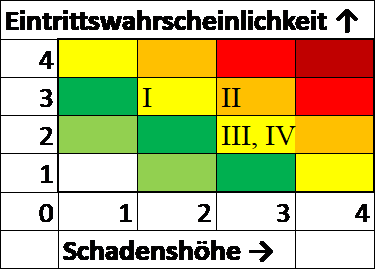
\includegraphics[width=0.4\textwidth]{Strom_Risiko_Akku_Ladung.png}
        \caption {Risikomatrix Antriebsenergie über die Schienen und Akku für die Systemsteuerung und Ladeschaltung für den Akku}
        \label{fig:strom_risikomatrix_akku_mitladung}
    \end{figure}

    Die zusätzlich nötige Schaltung erhöht die Kosten und die Schwierigkeit für die Umsetzung dieser Lösung. Um sicherzustellen, dass für den Antrieb auf der Strecke genügend Energie bleibt, muss die Schaltung so implementiert werden, dass der Akku nur geladen wird, wenn genügend Energie zur verfügung steht. Am besten wird der Ladevorgang während der schnellen Fahrt Komplett unterbrochen.

    
    \subsubsection{Entscheid}
    Mithilfe der Nutzwertanalyse in Abbildung \ref{fig:strom_nutzwertanalyse} konnte ein Entscheid getroffen werden.\\
    Die Stromversorgung alleine über die Schienen schneidete vorallem bei der Prozesssicherhiet schlecht ab. Das Risiko für Unterbrüche ist bei dieser Möglichkeit zu hoch.\\
    Mit einem zusätzlichen Akku kann dieses Risiko  minimiert werden. Auch die Umsetzung mit einem einfachen akku sollte kein Risiko darstellen.\\
    Die Möglichkeit einer zusätzlich Ladeschaltung ist dagegen um einiges Komplizierter und Aufwändiger. Dabei ist zu bedenken, dass der Ladevorgang entsprechend der verfügbaren Energie gesteuert werden müsste. Während der Fahrt soll die Gesamte Energie dem Antrieb zur Verfügung stehen und die Ladeschaltung muss inaktiv sein.
        
    \begin{figure}[H]
        \centering
        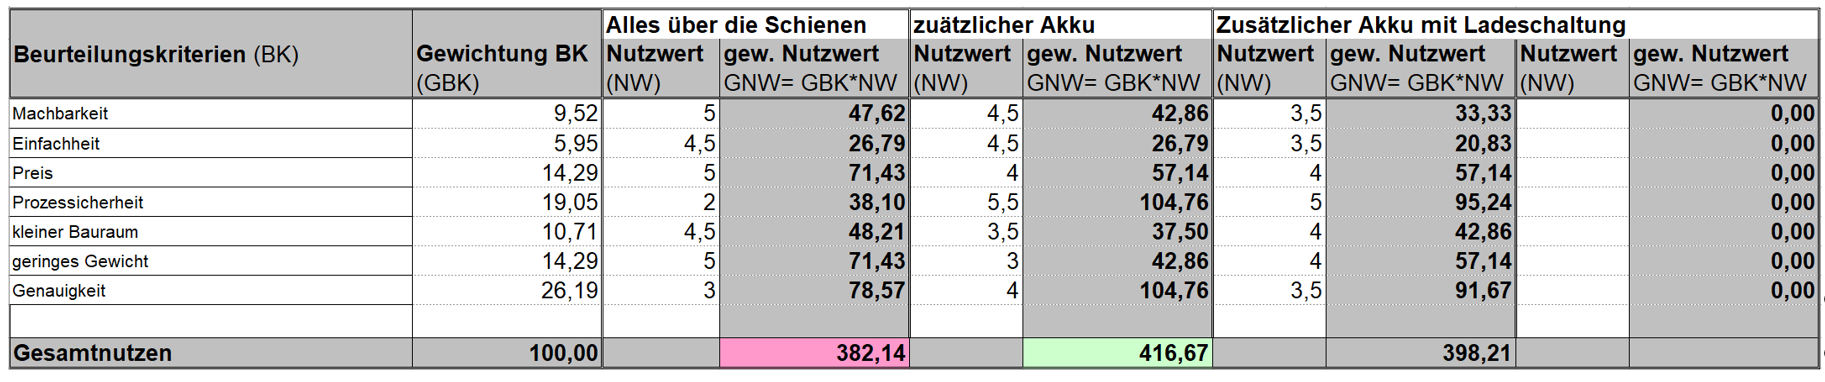
\includegraphics[width=1.0\textwidth]{Strom_Nutzwertanalyse.png}
        \caption {Nutzwertanalyse Antrieb}
        \label{fig:strom_nutzwertanalyse}
    \end{figure}

    Der Entscheid für die beste Möglichkeit fiel auf den zusätzlichen Akku ohne Ladeschaltung. Das Risiko eines Unterbruchs wäre ohne Akku zu gross. Was weiterhin zu beachten ist, ist dass der Akku genügend gross ausgelegt wird, da er nicht nur für den Wettbewerb reichen soll, sondern auch für längere Tests das System mit Strom versorgen kann.\\ 
    Die Möglichkeit einer Ladeschaltung wurde aufgrund der aufwändigeren Umsetzung zurückgestellt. Sie wird aber weiterhin verfolgt und kann zu einem späteren Zeitpunkt als Erweiterung noch umgesetzt werden.
    


    \end{document}